% =====================================================================
%  COMPANION to theory_v2: the logical chain, step-by-step derivations,
%  what goes in the main text, what goes in the extension.
%  Build: tectonic -X compile theory_companion.tex  (uses fig_release.pdf from make_figs_v2.py)
% =====================================================================
\documentclass[11pt,a4paper]{article}
\usepackage[a4paper,margin=2.2cm]{geometry}
\usepackage[T1]{fontenc}\usepackage[utf8]{inputenc}\usepackage{lmodern}
\usepackage{amsmath,amssymb,bm}
\usepackage{booktabs,array,longtable}
\usepackage{enumitem}
\usepackage{xcolor}
\usepackage{graphicx}
\usepackage{tikz}
\usetikzlibrary{arrows.meta,positioning,shapes.geometric,calc}
\usepackage{caption}
\captionsetup{font=small,labelfont=bf,width=0.92\textwidth}
\usepackage{tcolorbox}
\usepackage[hidelinks]{hyperref}
\colorlet{copper}{orange!80!black}
\newcommand{\muz}{\mu_0}\newcommand{\mum}{\mu_{\mathrm m}}\newcommand{\dd}{\mathrm{d}}\newcommand{\un}[1]{\,\mathrm{#1}}\newcommand{\Lag}{\mathcal L}
\newtcolorbox{stepbox}[1]{colback=blue!3,colframe=blue!45!black,boxrule=0.5pt,arc=2pt,left=5pt,right=5pt,top=3pt,bottom=3pt,title={#1},fonttitle=\bfseries\small}
\newtcolorbox{writebox}{colback=green!4,colframe=green!40!black,boxrule=0.5pt,arc=2pt,left=5pt,right=5pt,top=3pt,bottom=3pt,fontupper=\small,title=What to write in the essay,fonttitle=\bfseries\small}
\newtcolorbox{warnbox}{colback=red!4,colframe=red!50!black,boxrule=0.5pt,arc=2pt,left=5pt,right=5pt,top=3pt,bottom=3pt,fontupper=\small,title=Pitfalls,fonttitle=\bfseries\small}
\setlist{itemsep=1pt,topsep=2pt}
\title{\vspace{-1.5em}Theory companion: how the pieces fit together\\[2pt]\large Coupled magnetic--mechanical oscillator --- derivations, dependencies, and what goes where}
\author{}\date{}
\begin{document}\maketitle\vspace{-2.5em}

\section*{0. First: why the beat envelope in the earlier figure was ``shifted''}
It was a sign error in the \emph{plotting script}, not in the physics; the figure is now regenerated (Figure~\ref{fig:release} below). The lesson is worth keeping because it is exactly the calculation you need for the beat-minimum test. With $x_1=\tfrac12(\eta_0\cos\omega_1t-\xi_0\cos\omega_2t)$, the amplitude of the fast oscillation is
\[
|x_1|_{\rm env}=\tfrac12\sqrt{\eta_0^2+\xi_0^2-2\eta_0\xi_0\cos(\omega_2-\omega_1)t}\,,
\]
and for a hold-and-release start $\eta_0=-(A+x_{20})<0$ while $\xi_0=A-x_{20}>0$. So at $t=0$ the square root is $\sqrt{(|\eta_0|+\xi_0)^2}$, i.e.\ the envelope starts at its \emph{maximum} $A$ (the spring was just released from $-A$) and reaches its first \emph{minimum} $x_{20}$ at $t=T_{\rm beat}/2$. The old script had $+2\eta_0\xi_0$, which put the minimum at $t=0$ --- a quarter-beat shift. Rule: derive the envelope from the actual signs of $\eta_0$ and $\xi_0$, never from ``$\cos+\cos$'' memory.

\section*{1. The chain of reasoning (main text)}
\begin{figure}[h]\centering
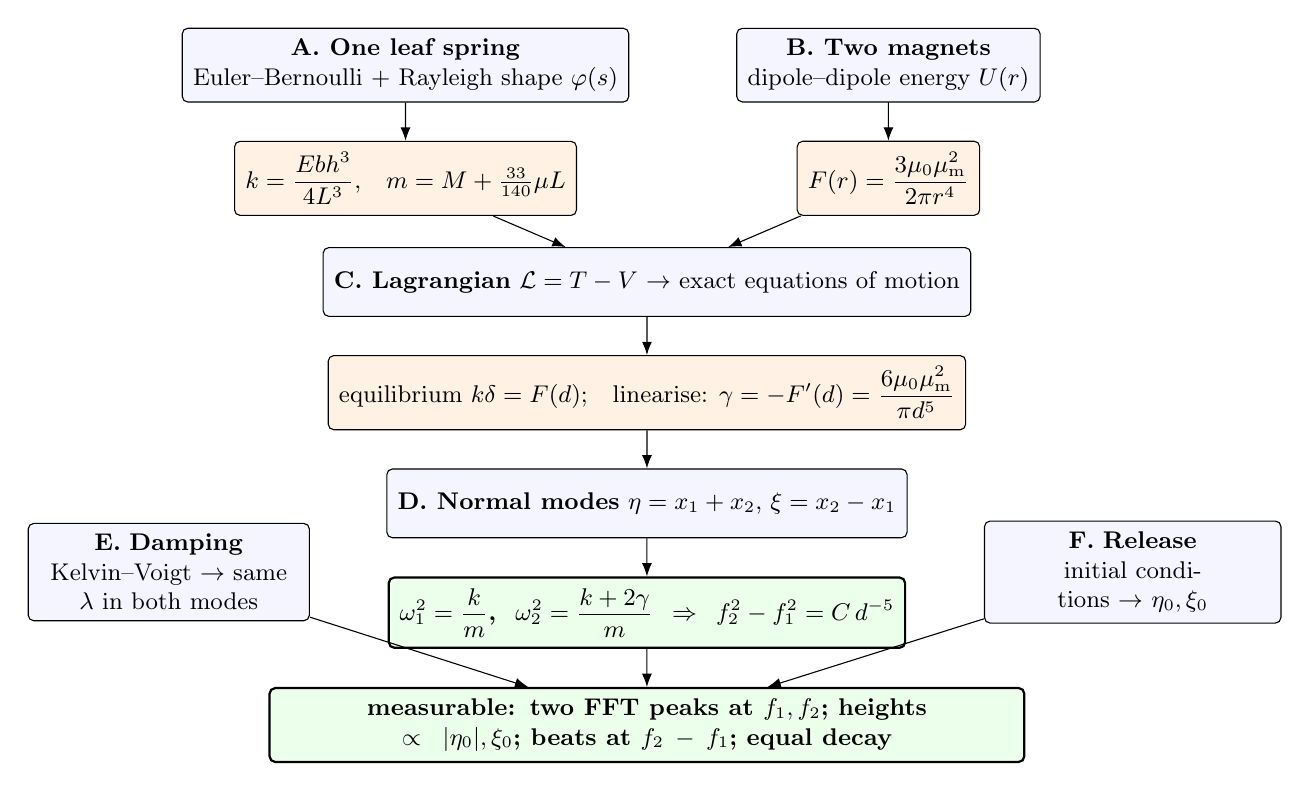
\begin{tikzpicture}[>=Latex,node distance=5mm and 8mm,scale=0.97,transform shape,
  box/.style={draw,rounded corners=2pt,fill=blue!4,align=center,font=\small,inner sep=4pt,minimum height=9mm},
  res/.style={draw,rounded corners=2pt,fill=orange!10,align=center,font=\small,inner sep=4pt,minimum height=9mm},
  keyres/.style={draw,thick,rounded corners=2pt,fill=green!8,align=center,font=\small\bfseries,inner sep=4pt,minimum height=9mm}]
\node[box] (beam) {\textbf{A. One leaf spring}\\ Euler--Bernoulli + Rayleigh shape $\varphi(s)$};
\node[res,below=of beam] (km) {$k=\dfrac{Ebh^3}{4L^3}$,\quad $m=M+\tfrac{33}{140}\mu L$};
\node[box,right=14mm of beam] (dip) {\textbf{B. Two magnets}\\ dipole--dipole energy $U(r)$};
\node[res,below=of dip] (F) {$F(r)=\dfrac{3\muz\mum^2}{2\pi r^4}$};
\node[box,below=9mm of $(km)!0.5!(F)$] (lag) {\textbf{C. Lagrangian} $\Lag=T-V$ $\to$ exact equations of motion};
\node[res,below=of lag] (eq) {equilibrium $k\delta=F(d)$;\quad linearise: $\gamma=-F'(d)=\dfrac{6\muz\mum^2}{\pi d^5}$};
\node[box,below=of eq] (modes) {\textbf{D. Normal modes} $\eta=x_1+x_2$, $\xi=x_2-x_1$};
\node[keyres,below=of modes] (main) {$\omega_1^2=\dfrac km$,\ \ $\omega_2^2=\dfrac{k+2\gamma}{m}$\ \ $\Rightarrow$\ \ $f_2^2-f_1^2=C\,d^{-5}$};
\node[box,left=10mm of modes,yshift=-9mm,text width=34mm] (damp) {\textbf{E. Damping}\\ Kelvin--Voigt $\to$ same $\lambda$ in both modes};
\node[box,right=10mm of modes,yshift=-9mm,text width=36mm] (rel) {\textbf{F. Release}\\ initial conditions $\to$ $\eta_0,\xi_0$};
\node[keyres,below=of main,text width=96mm] (test) {measurable: two FFT peaks at $f_1,f_2$; heights $\propto|\eta_0|,\xi_0$; beats at $f_2-f_1$; equal decay};
\draw[->] (beam)--(km); \draw[->] (dip)--(F); \draw[->] (km)--(lag); \draw[->] (F)--(lag); \draw[->] (lag)--(eq); \draw[->] (eq)--(modes); \draw[->] (modes)--(main); \draw[->] (main)--(test);
\draw[->] (damp)--(test); \draw[->] (rel)--(test);
\end{tikzpicture}
\caption{Every box feeds the next; nothing is assumed that is not derived above it. The extension (Section~2) branches off at C: keep $F(r)$ exact instead of linearising.}
\end{figure}

\subsection*{A. One leaf spring $\to$ $k$ and $m$}
\begin{stepbox}{A1. Shape function (the one modelling assumption)}
The strip vibrates in its lowest mode, whose shape is taken as the static deflection curve under a tip load:
\[ y(s,t)=x(t)\,\varphi(s),\qquad \varphi(s)=\frac{3Ls^2-s^3}{2L^3}. \]
Check the boundary conditions: $\varphi(0)=0$ (clamped), $\varphi'(0)=0$ (clamped, no slope), $\varphi(L)=1$ (tip moves by $x$), $\varphi''(L)=0$ (no bending moment at a free end). One function of $s$ times one function of $t$: the beam becomes a single coordinate $x(t)$.
\end{stepbox}
\begin{stepbox}{A2. Energies $\to$ $m$ and $k$}
Kinetic energy of the strip: each element $\mu\,\dd s$ moves at $\dot x\varphi(s)$, so
\[ T_{\rm beam}=\tfrac12\mu\dot x^2\int_0^L\varphi^2\,\dd s=\tfrac12\Bigl(\tfrac{33}{140}\mu L\Bigr)\dot x^2. \]
Elastic energy of a bent beam is $\tfrac12EI\int(y'')^2\dd s$ (curvature $y''$, flexural rigidity $EI$, $I=bh^3/12$):
\[ V_{\rm beam}=\tfrac12EIx^2\int_0^L(\varphi'')^2\dd s=\tfrac12\Bigl(\frac{3EI}{L^3}\Bigr)x^2 . \]
The two integrals are $\int_0^L\varphi^2\dd s=\frac{33}{140}L$ and $\int_0^L\varphi''^2\dd s=3/L^3$ (with $\varphi''=3(L-s)/L^3$). Adding the magnet ($\tfrac12M\dot x^2$):
\[ \boxed{m=M+\tfrac{33}{140}\mu L,\qquad k=\frac{3EI}{L^3}=\frac{Ebh^3}{4L^3}} \]
\textit{Used in:} C (as the $T$ and $V$ of each spring). \textit{By-products:} tip rotation $\theta=\varphi'(L)x=3x/2L$ (used in B for the tilt correction); the $\tfrac{33}{140}$ is why the magnet mass alone is not $m$.
\end{stepbox}
\begin{warnbox}
$T_{\rm beam}=\tfrac{33}{280}\mu L\dot x^2$ and $m_{\rm eff}=\tfrac{33}{140}\mu L$ are the same statement ($T=\tfrac12 m_{\rm eff}\dot x^2$). Quote one, not both as if different. $k=3EI/L^3$ is the tip stiffness of a cantilever --- don't confuse with $48EI/L^3$ (simply supported beam).
\end{warnbox}

\subsection*{B. Two magnets $\to$ $F(r)$}
\begin{stepbox}{B1. Dipole energy}
Magnet 2 (moment $\bm\mu_2$) in the field $\bm B_1$ of magnet 1: $U=-\bm\mu_2\cdot\bm B_1$ with $\bm B_1=\dfrac{\muz}{4\pi r^3}\bigl[3(\bm\mu_1\!\cdot\!\hat{\bm r})\hat{\bm r}-\bm\mu_1\bigr]$, hence
\[ U=\frac{\muz}{4\pi r^3}\bigl[\bm\mu_1\!\cdot\!\bm\mu_2-3(\bm\mu_1\!\cdot\!\hat{\bm r})(\bm\mu_2\!\cdot\!\hat{\bm r})\bigr]. \]
Like poles facing on a common axis: $\bm\mu_1=\mum\hat{\bm r}$, $\bm\mu_2=-\mum\hat{\bm r}$, so $\bm\mu_1\!\cdot\!\bm\mu_2=-\mum^2$ and $(\bm\mu_1\!\cdot\!\hat{\bm r})(\bm\mu_2\!\cdot\!\hat{\bm r})=-\mum^2$:
\[ U(r)=\frac{\muz}{4\pi r^3}\bigl[-\mum^2+3\mum^2\bigr]=\frac{\muz\mum^2}{2\pi r^3}>0 . \]
\end{stepbox}
\begin{stepbox}{B2. Force and its slope}
\[ F(r)=-\frac{\dd U}{\dd r}=\frac{3\muz\mum^2}{2\pi r^4}\ (\text{repulsive}),\qquad \gamma(r)\equiv-\frac{\dd F}{\dd r}=\frac{6\muz\mum^2}{\pi r^5}=\frac{4F(r)}{r}. \]
\textit{Used in:} C (equilibrium uses $F(d)$; linearisation uses $\gamma$). \textit{Tilt (optional, one sentence):} with the tips rotated by $\theta_i=3x_i/2L$ the bracket becomes $2\cos\theta_1\cos\theta_2-\sin\theta_1\sin\theta_2$; expanding to second order changes both mode frequencies by relative amounts $\lesssim\tfrac{9}{32}\frac{\gamma}{k}(d/L)^2<10^{-3}$. Say it is negligible and move on.
\end{stepbox}

\subsection*{C. Lagrangian $\to$ equations of motion, equilibrium, linearisation}
\begin{stepbox}{C1. Lagrangian and exact equations}
Coordinates: $x_1,x_2$ = tip displacements from the springs' \emph{unstressed} positions, both positive to the right; separation $r=d_0+x_2-x_1$.
\[ \Lag=\tfrac12m(\dot x_1^2+\dot x_2^2)-\tfrac12k(x_1^2+x_2^2)-U(d_0+x_2-x_1). \]
$\dfrac{\dd}{\dd t}\dfrac{\partial\Lag}{\partial\dot x_i}=\dfrac{\partial\Lag}{\partial x_i}$ with $\partial U/\partial x_1=-U'(r)=+F$, $\partial U/\partial x_2=U'(r)=-F$:
\[ m\ddot x_1=-kx_1-F(r),\qquad m\ddot x_2=-kx_2+F(r). \]
(Read: the repulsion pushes 1 to the left and 2 to the right. Exact within the dipole and one-mode assumptions.)
\end{stepbox}
\begin{stepbox}{C2. Equilibrium}
Set accelerations to zero: $kx_1=-F$, $kx_2=+F$ $\Rightarrow$ each spring bent outwards by $\delta=F(d)/k$, separation $d=d_0+2\delta$. \textit{This $d$ (with magnets mounted) is the measured variable.}
\end{stepbox}
\begin{stepbox}{C3. Linearisation}
Now let $x_1,x_2$ be displacements from equilibrium, so $r=d+\xi$ with $\xi=x_2-x_1$. Taylor: $F(d+\xi)\simeq F(d)+F'(d)\xi=F(d)-\gamma\xi$. Insert; the constant $F(d)$ cancels against $k\delta$:
\[ \boxed{m\ddot x_1=-kx_1+\gamma(x_2-x_1),\qquad m\ddot x_2=-kx_2-\gamma(x_2-x_1)} \]
Interpretation: a compressed spring of stiffness $\gamma$ between the magnets. \textit{Validity:} $|\xi|\ll d$; the neglected term is $\tfrac12F''(d)\xi^2=\tfrac{5\gamma}{2d}\xi^2$ --- this is the entry point of the extension.
\end{stepbox}

\subsection*{D. Normal modes $\to$ the tested relation}
\begin{stepbox}{D1. Decoupling}
Add and subtract the two equations:
\[ m\ddot\eta=-k\eta,\qquad m\ddot\xi=-(k+2\gamma)\xi,\qquad \eta\equiv x_1+x_2,\ \xi\equiv x_2-x_1. \]
Two independent harmonic oscillators:
\[ \boxed{\omega_1^2=\frac km\quad(\text{in-phase: }\xi=0),\qquad \omega_2^2=\frac{k+2\gamma}m\quad(\text{anti-phase: }\eta=0)} \]
Why $2\gamma$: in the anti-phase mode each magnet moves $a$, the gap changes by $2a$, the extra force on each is $\gamma\cdot2a$.
\end{stepbox}
\begin{stepbox}{D2. Eliminate the unknown spring}
\[ \omega_2^2-\omega_1^2=\frac{2\gamma}{m}\ \Rightarrow\ f_2^2-f_1^2=\frac{\gamma}{2\pi^2m}=\frac{6\muz\mum^2}{2\pi^3m}\,d^{-5}=\underbrace{\frac{3\muz\mum^2}{\pi^3m}}_{C}\,d^{-5}. \]
\[ \boxed{\ln(f_2^2-f_1^2)=\ln C-5\ln d} \]
Predictions to test: (i) $f_1$ independent of $d$ and equal to the single-spring frequency; (ii) gradient $-5$; (iii) intercept gives $C$, i.e.\ $\mum$ if $m$ is known. Everything unknown about the spring has dropped out of the gradient.
\end{stepbox}

\subsection*{E. Damping (Kelvin--Voigt) $\to$ why the frequencies are safe and what the envelope tests}
\begin{stepbox}{E1. From the material law to the mode equations}
Kelvin--Voigt solid: $\sigma=E(\varepsilon+\tau_{\rm v}\dot\varepsilon)$. Integrated over the cross-section, the bending moment becomes $EI(y''+\tau_{\rm v}\dot y'')$, so the beam equation is
\[ \mu\ddot y=-EI\bigl(y''''+\tau_{\rm v}\dot y''''\bigr). \]
Insert $y=x(t)\varphi(s)$ and project onto $\varphi$ (multiply by $\varphi$, integrate --- the same two integrals as in A2): $m\ddot x=-kx-k\tau_{\rm v}\dot x$. Air drag on the magnet adds $-c_{\rm a}\dot x$. Both are linear in $\dot x$ and identical for identical springs, so in the mode equations
\[ \ddot\eta+2\lambda\dot\eta+\omega_1^2\eta=0,\qquad \ddot\xi+2\lambda\dot\xi+\omega_2^2\xi=0,\qquad 2\lambda=\frac{k\tau_{\rm v}+c_{\rm a}}{m}. \]
\end{stepbox}
\begin{stepbox}{E2. Consequences}
Solutions $e^{-\lambda t}\cos(\omega_i't+\phi)$ with $\omega_i'=\sqrt{\omega_i^2-\lambda^2}$. With $\tau_d=1/\lambda\approx21\un{s}$ and $\omega\approx41\un{s^{-1}}$: $\lambda/\omega\approx10^{-3}$, frequency shift $\lambda^2/2\omega^2\approx10^{-6}$ --- negligible. Peak full width $\approx1/\pi\tau_d\approx15\un{mHz}$. Both modes decay at the \emph{same} rate $\Rightarrow$ ratio of the two FFT peaks and ratio of beat minima to maxima are constant in time. A relative-motion damping (eddy currents between the magnets) would break this --- a testable statement.
\end{stepbox}

\subsection*{F. The release $\to$ what the record should look like}
\begin{stepbox}{F1. Initial conditions}
Spring 1 held at $x_1=-A$, spring 2 free and at rest: from the static form of C3, $kx_2=\gamma(x_1-x_2)\Rightarrow x_2=-\dfrac{\gamma}{k+\gamma}A\equiv-x_{20}$. Both released from rest, so only cosines appear:
\[ \eta_0=x_1(0)+x_2(0)=-(A+x_{20}),\qquad \xi_0=x_2(0)-x_1(0)=A-x_{20}. \]
\end{stepbox}
\begin{stepbox}{F2. Motion, spectrum, beats}
\[ x_1=\tfrac12(\eta_0\cos\omega_1t-\xi_0\cos\omega_2t),\qquad x_2=\tfrac12(\eta_0\cos\omega_1t+\xi_0\cos\omega_2t). \]
\emph{Spectrum:} two lines at $f_1,f_2$ in \emph{both} records, heights $\tfrac12|\eta_0|$ and $\tfrac12\xi_0$, ratio
\[ \frac{\xi_0}{|\eta_0|}=\frac{A-x_{20}}{A+x_{20}}=\frac{k}{k+2\gamma}=\Bigl(\frac{f_1}{f_2}\Bigr)^2 . \]
(Algebra: $A-x_{20}=A\frac{k}{k+\gamma}$, $A+x_{20}=A\frac{k+2\gamma}{k+\gamma}$.)\quad
\emph{Beats:} write $x_1=\Re\bigl[\tfrac12(\eta_0e^{i\omega_1t}-\xi_0e^{i\omega_2t})\bigr]$; the modulus of the bracket is the envelope,
\[ |x_1|_{\rm env}=\tfrac12\sqrt{\eta_0^2+\xi_0^2-2\eta_0\xi_0\cos(\omega_2-\omega_1)t}\ \in\bigl[\,x_{20},\,A\,\bigr],\qquad T_{\rm beat}=\frac1{f_2-f_1}. \]
Maximum $A$ at $t=0$ (just released), minimum $x_{20}$ at $t=T_{\rm beat}/2$; spring 2 is the mirror image (its envelope has $+2\eta_0\xi_0$): energy exchange. Three independent handles on $\gamma/k$: peak ratio, beat minimum, and $f_2/f_1$ itself.
\end{stepbox}
\begin{figure}[h]\centering
\includegraphics[width=0.95\textwidth]{fig_release.pdf}
\caption{Corrected figure: envelope from F2 with the actual signs of $\eta_0,\xi_0$; it starts at $A$ and first touches $x_{20}$ at $T_{\rm beat}/2$; the second spring is a quarter-beat behind.}\label{fig:release}\end{figure}

\begin{writebox}
Main-text theory, in this order and roughly this length (about 3--4 pages with figures):
\begin{enumerate}
\item \textbf{One spring} (½ page + Fig.~``geometry of the leaf spring''): A1--A2 boxed results; one sentence on why Rayleigh's shape is adequate ($<0.2\,\%$ error with a tip mass).
\item \textbf{Two magnets} (½ page + Fig.~``equilibrium and coordinates''): B1--B2; state $F\propto r^{-4}$ and $\gamma=4F/d$.
\item \textbf{Lagrangian and small oscillations} (¾ page): C1--C3; the boxed linear equations; state the validity condition $|\xi|\ll d$ and that the extension removes it.
\item \textbf{Normal modes} (¾ page + Fig.~``two modes''): D1--D2 with the key box $f_2^2-f_1^2=Cd^{-5}$ and the three predictions.
\item \textbf{Damping and release} (¾ page + Fig.~\ref{fig:release}): E2 and F2 as statements with the two-line derivations; the summary table of predictions vs.\ tests.
\end{enumerate}
Every box's ``\textit{Used in}'' line is the sentence that links the paragraphs --- write those transitions explicitly; that is what makes the theory read as an argument rather than a list.
\end{writebox}

\newpage
\section*{2. Extension: the non-linear force law}
\begin{stepbox}{X1. Exact mode equations (branch off at C1, do not linearise)}
Subtract and add the exact equations of C1, with $x_i$ measured from equilibrium ($r=d+\xi$):
\[ m\ddot\eta=-k\eta\ \ (\text{exactly}),\qquad m\ddot\xi=-k\xi+2\bigl[F(d+\xi)-F(d)\bigr]. \]
Sign check: $\xi>0$ (further apart) $\Rightarrow F(d+\xi)<F(d)$ $\Rightarrow$ bracket negative $\Rightarrow$ restoring. Linear limit: $2F'(d)\xi=-2\gamma\xi$ ✓. \textbf{Key statement for the essay:} the centre of mass is exactly harmonic at $\omega_1$ whatever the force law, because the magnetic force is internal; all non-linearity is in the relative coordinate --- so $f_1$ can never depend on amplitude, and only $f_2$ can.
\end{stepbox}
\begin{stepbox}{X2. Expand}
$F(d+\xi)=F(d)(1+u)^{-4}$, $u=\xi/d$, and $(1+u)^{-4}=1-4u+10u^2-20u^3+\dots$; with $2F(d)/d=\gamma/2$:
\[ \ddot\xi+\omega_2^2\xi=\frac{\gamma}{m}\Bigl[5\frac{\xi^2}{d}-10\frac{\xi^3}{d^2}+\dots\Bigr]=\omega_2^2\,g\Bigl[5\frac{\xi^2}{d}-10\frac{\xi^3}{d^2}\Bigr],\qquad g\equiv\frac{\gamma}{k+2\gamma}=\frac{\gamma/m}{\omega_2^2}. \]
Two small parameters: $g$ (how magnetic the anti-phase stiffness is; $0.13$ at $24.5\un{mm}$) and $\xi/d$ (amplitude).
\end{stepbox}
\begin{stepbox}{X3. Solve by successive approximation (Lindstedt--Poincar\'e)}
Try $\xi=a\cos\omega t+\text{(small corrections)}$ and use $\cos^2=\tfrac12(1+\cos2\omega t)$, $\cos^3=\tfrac14(3\cos\omega t+\cos3\omega t)$.
\emph{Second order} ($\xi^2$ term drives $0$ and $2\omega$): $\xi_2=\dfrac{5ga^2}{2d}-\dfrac{5ga^2}{6d}\cos2\omega t$ (the $\cos2\omega t$ response is divided by $\omega_2^2-4\omega^2\simeq-3\omega_2^2$, hence the $1/6$ and the minus sign).
\emph{Third order}: the $\cos\omega t$ terms produced by $\xi^3$ and by $\xi_1\xi_2$ would grow without bound (resonant) unless the frequency shifts; demanding they cancel gives
\[ \boxed{\frac{\omega-\omega_2}{\omega_2}=\Bigl(\frac ad\Bigr)^2\Bigl[\frac{15g}{4}-\frac{125g^2}{12}\Bigr]},\qquad \xi_3\ni\Bigl(\frac{5g}{16}+\frac{25g^2}{48}\Bigr)\frac{a^3}{d^2}\cos3\omega t . \]
(All four coefficients checked by computer algebra and by direct numerical integration --- agreement to 2 \% at $a/d=0.17$.)
\end{stepbox}
\begin{stepbox}{X4. What it predicts, numerically ($d=24.5\un{mm}$, $A=5\un{mm}$, pilot constants)}
$g=0.13$, $a\simeq\xi_0=4.2\un{mm}$: $f_2$ up by $0.9\,\%$ ($0.07\un{Hz}$ --- comparable to a frequency bin of a 10 s record, so real but small); second harmonic $2f_2$ at $1.9\,\%$ of the fundamental in the spectrum of $\xi$; mean separation increased by $0.24\un{mm}$; $f_1$ unchanged. With $A=10\un{mm}$ multiply the shift by 4. In a decaying record the FFT sees a time-average, roughly $0.15$--$0.2$ of the initial-amplitude shift.
\end{stepbox}
\begin{stepbox}{X5. Internal resonance (the ``critical value'')}
If $\omega_2=2\omega_1$, the $2\omega_2$-driven terms are far from resonance but the $\eta$--$\xi$ cross terms (from tilt or any small asymmetry) become resonant and energy moves between modes: the 2:1 internal resonance other groups mention. Condition: $1+2\gamma/k=4\Rightarrow2\gamma/k=3\Rightarrow d^*=(C/3f_1^2)^{1/5}\approx16\un{mm}$ --- below the smallest achievable $d$ and outside the dipole regime. State that it is not met and that this is why the linear model stays valid throughout the range.
\end{stepbox}
\begin{writebox}
Extension / evaluation (1--1½ pages): X1 (three lines --- the exact-$\eta$ statement is the strongest single sentence in the extension), X2 (the expanded equation), X3 boxed results only, X4 as a table of numbers at your two smallest $d$, X5 as one paragraph. Then use it: (i) explain any upward bend of the ln--ln residuals at small $d$; (ii) justify the amplitude control; (iii) if you have an amplitude series at fixed $d$, plot $f_2$ against $\xi_0^2$ --- the gradient tests X3 directly; (iv) look for the $2f_2$ line in the spectrum of $\xi$ (log scale) as an optional check.
\end{writebox}

\section*{3. Checks performed (so you can quote them)}
\begin{center}\footnotesize
\begin{tabular}{@{}p{5.4cm}p{5.0cm}p{5.0cm}@{}}\toprule
quantity & result & how checked\\ \midrule
$\int_0^L\varphi^2\dd s$, $\int_0^L\varphi''^2\dd s$, $\varphi'(L)$ & $\tfrac{33}{140}L$, $3/L^3$, $3/2L$ & symbolic integration\\
Rayleigh $\omega_0$ vs exact cantilever+tip mass & $+1.5\,\%$ ($M=0$), $<0.2\,\%$ ($M>\tfrac12\mu L$) & transcendental root of exact solution\\
$F=3\muz\mum^2/2\pi r^4$, $\gamma=6\muz\mum^2/\pi r^5=4F/r$ & ✓ & symbolic differentiation\\
tilt correction to $\omega_1^2,\omega_2^2$ & $-\tfrac{9}{32}\tfrac{\gamma}{k}(d/L)^2$, $-\tfrac{3}{32}g(d/L)^2$ & 2nd-order series of the tilted-dipole energy\\
$(1+u)^{-4}$ coefficients & $1,-4,10,-20$ & series\\
Lindstedt coefficients ($c_0,c_2,c_3,\Delta\omega$) & as in X3 & symbolic projection onto $1,\cos2\tau,\cos\tau,\cos3\tau$\\
X3 vs numerical integration & shift, $c_2$, $c_3$, $c_0$ within 2--5 \% up to $a/d=0.17$ & \texttt{nonlinear\_check.py}\\
envelope of $x_1$ & starts at $A$, minimum $x_{20}$ at $T_{\rm beat}/2$ & Hilbert transform of the synthetic signal\\
peak ratio $\xi_0/|\eta_0|=(f_1/f_2)^2$ & $0.737=0.737$ at $24.5\un{mm}$ & synthetic spectrum\\ \bottomrule
\end{tabular}
\end{center}

\begin{warnbox}
\begin{itemize}
\item Sign conventions: both $x_i$ positive to the right; $\xi=x_2-x_1$ is the \emph{change of separation}; $\eta_0<0$ for a leftward pull. Keep one convention for the whole essay.
\item $f_{\rm beat}=f_2-f_1$ (period of the envelope swellings), not $(f_2-f_1)/2$ (period of the amplitude \emph{sign} pattern). Your RQ uses the former.
\item Kelvin--Voigt is a statement about the \emph{strip}; it predicts equal $\lambda$ for both modes only because the strips are identical and the coupling is conservative. Say that explicitly.
\item $C$ contains $m$ (the effective mass), not $M$; and $\mum$ is the dipole moment of one magnet ($=B_r V/\muz$ for a uniformly magnetised block, if you want a data-sheet estimate).
\item ``The dipole approximation'' is an assumption of B, not of C or D; if the exponent comes out below 5, the suspect is B (finite magnet size), not the normal-mode algebra.
\end{itemize}
\end{warnbox}
\end{document}
